% !TeX spellcheck = de_DE
\documentclass[12pt,bibstyle=none,pagenumberinfooter]{ifmdocument}


%general settings
\author{...}
\title{Einf\"uhrung in moofeKIT}
\date{\the\day.\the\month.\the\year}
\headerblock{%
	{\bfseries\normalsize Institut für Mechanik}\\[0.2em]
	\thetitle\\
	%\theauthor, \thedate
	\thedate
}

%usercommands
%-----------------------------------------------------------------------
%special user commands and packages
%-----------------------------------------------------------------------
%ENTER USER COMMANDS AND PACKAGES HERE

\usepackage{url}
\def\UrlBreaks{\do\a\do\b\do\c\do\d\do\e\do\f\do\g\do\h\do\i\do\j\do\k\do\l\do\m\do\n\do\o\do\p\do\q\do\r\do\s\do\t\do\u\do\v\do\w\do\x\do\y\do\z\do\0\do\1\do\2\do\3\do\4\do\5\do\6\do\7\do\8\do\9\do\-}%

%\usepackage[hyphens]{url}
%\usepackage{hyperref}
%-----------------------------------------------------------------------
%standard user commands and additional packages (most in ifmthesis.cls)
\usepackage[edges]{forest}
%-----------------------------------------------------------------------
%assembly symbol (simple)
\DeclareMathOperator*{\assem}{\text{\Large\ensuremath{\mathbf{\textsf A}}}}
\DeclareMathOperator*{\assemtext}{\text{{\ensuremath{\mathbf{\textsf A}}}}}
%functions, operators
\newcommand{\cof}{\ensuremath{\operatorname{cof}}}
\renewcommand{\div}{\ensuremath{\operatorname{div}}}
\newcommand{\Div}{\ensuremath{\operatorname{Div}}}
\newcommand{\Grad}{\ensuremath{\operatorname{Grad}}}
\newcommand{\grad}{\ensuremath{\operatorname{grad}}}
\newcommand{\Curl}{\ensuremath{\operatorname{Curl}}}
\newcommand{\curl}{\ensuremath{\operatorname{curl}}}
\newcommand{\tr}{\ensuremath{\operatorname{tr}}}
\newcommand{\sign}{\ensuremath{\operatorname{sign}}}
%differential signs
\renewcommand{\d}[1][]{\ensuremath{\,\mathrm{d}#1}}
\newcommand{\D}[1][]{\ensuremath{\mathrm{D}#1}}
\newcommand{\nablaq}[1]{\ensuremath{\nabla_{\hspace{-0.5ex}\mbox{\begin{scriptsize}\vec{#1}\end{scriptsize}}}}\hspace{0.1ex}}
%useful for continuum mechanics fem
\renewcommand{\phi}{\varphi}
\renewcommand{\epsilon}{\varepsilon}
\newcommand{\body}{\ensuremath{\mathcal{B}}}
\newcommand{\refgeb}{\hat{\Omega}}
\newcommand{\he}{\ensuremath{^{h,e}}}
\newcommand{\transp}{\mathrm{T}}
%misc
\newcommand{\degree}{\textdegree}
\def\clap#1{\hbox to 0pt{\hss#1\hss}}
\def\mathclap{\mathpalette\mathclapinternal}
\def\mathclapinternal#1#2{\clap{$\mathsurround=0pt#1{#2}$}}
\newcommand{\matlab}{\textsc{Matlab}}
%floats
\newcommand{\picfontsize}{\small}
\newenvironment{myfigure}{\begin{figure}[htb]\centering\picfontsize}{\end{figure}}
\newenvironment{mytable}{\begin{table}[htb]\centering}{\end{table}}
\hyphenation{in-te-gra-ble in-te-gra-bil-i-ty}% Silbentrennung
%dot and comma to end equations
\newcommand{\eqcomma}{\ensuremath{\text{,}}}
\newcommand{\eqdot}{\ensuremath{\text{.}}}
%vec and tens
\renewcommand{\vec}[1]{\ensuremath{\mbox{\boldmath $\mathrm{#1}$}}}
\newcommand{\tens}[1]{\vec{#1}}
%checkmark and xmark
\usepackage{bbding}
\newcommand{\cmark}{\Checkmark}
\newcommand{\xmark}{\XSolidBrush}
%Tensorcrossproduct
\usepackage{stackengine}
\def\stacktype{L}
\stackMath
\def\newhash{\mathrel{\abovebaseline[-.9ex]{\rotatebox{45}{\stackon[0pt]{%
					\stackon[0pt]{\rule[.28em]{.8em}{.045em}}{\rule[.67em]{.8em}{.045em}}%
				}{\rule[.1em]{.045em}{.8em}\rule{.3em}{0pt}\rule[.1em]{.045em}{.8em}}}}}}
\newcommand{\hhash}{\scalebox{0.75}{\raisebox{.7ex}{$\newhash$}}} 

% specific commands
\usepackage{float}
\usepackage{dirtree}
\newcommand{\voigt}{\mathrm{v}}
\renewcommand{\he}{\ensuremath{^{\mathrm{h},e}}}
\newcommand{\code}[1]{\texttt{#1}}

\begin{document}
	\maketitle
\section{Ein einführendes Beispiel}
Die wichtigsten Funktionen von moofeKIT sollen anhand eines numerischen Beispiels erläutert werden. Dazu betrachten wir die in Abbildung \ref{fig:cooksMembrane} dargestellte ebene Cooks-Membran, welche auch in der 12. \"Ubung der Lehrveranstaltung Grundlagen Finite Elemente untersucht wird. Als Materialparameter seien der Elastizit\"atsmodul $E=100$ und die Querkontraktionszahl $\nu=0.2$ gegeben.

\begin{myfigure}
	{
		\psfrag{1}[c][c]{\footnotesize $16$}
		\psfrag{2}[c][c]{\footnotesize$44$}
		\psfrag{3}[c][c]{\footnotesize$\vec{F}$}
		\psfrag{4}[c][c]{\footnotesize $\Omega$}
		\psfrag{5}[c][c]{\footnotesize$48$}
		\psfrag{6}[l][l]{\footnotesize $E,\,\nu$}
		\includegraphics[width=0.4\textwidth]{cooksMembrane}
	}
	\caption{grafische Darstellung der Cooks-Membran}
	\label{fig:cooksMembrane}
\end{myfigure}
Dieses numerische Beispiel ist bereits in moofeKIT implementiert und wird in den nachfolgenden Abschnitten detailliert erklärt. Im Gegensatz zum Beispiel aus der Übung wird die Last $\vec{F}$ in unserem Fall jedoch nicht von Anfang an voll aufgebracht, sondern schrittweise über insgesamt fünf Zeitschritte hinweg gesteigert (inkrementelle Laststeigerung). 

\subsection{Theoretische Grundlagen: Von der schwachen Form zum Gleichungssystem}
Zur Rekapitulation sollen in diesem Abschnitt die wichtigsten Gleichungen wiederholt werden. Wir gehen von einem statischen Problem aus, weshalb die schwache Form 
\begin{gather*}
	\int_{\Omega}\!\nabla\vec{v}:\vec{\sigma}\, \d V = \int_{\Omega}\!\vec{v}\cdot\vec{b}\, \d V + \int_{\partial\Omega_\sigma}\!\vec{v}\cdot \vec{\bar{t}}\, \d A
\end{gather*}
unter Verwendung der Randbedingungen aus den lokalen statischen Feldgleichungen hergeleitet werden kann. Dabei werden mit $\vec{v}$ die vektorwertigen Testfunktionen und mit $\Omega$ das gegebene Gebiet bezeichnet. Mit dem Hookeschen Gesetz in Voigtscher Notation $\vec{\sigma}^\voigt = \vec{D}\vec{\epsilon}^\voigt(\vec{u})$ kann die schwache Form alternativ auch durch
\begin{gather*}
	\int_{\Omega}\!\vec{\epsilon}^\voigt(\vec{v})^\transp\vec{D}\vec{\epsilon}^\voigt(\vec{u})\, \d V = \int_{\Omega}\!\vec{v}\cdot\vec{b}\, \d V + \int_{\partial\Omega_\sigma}\!\vec{v}\cdot \vec{\bar{t}}\, \d A
\end{gather*}
dargestellt werden.
%Differentialgleichung: 
%\begin{gather*}
%	\div \vec{\sigma} + \vec{b} = \vec{0} 
%\end{gather*}
%Randbedingungen: 
%\begin{alignat*}{2}
%	\vec{u} &= \vec{0}\quad &&\text{Dirichletrand}\\
%	\vec{\sigma}\vec{n}&=\vec{F}\quad &&\text{Neumannrand}
%\end{alignat*}
In diesem Beispiel wollen wir f\"ur die FE-Approximation das biquadratische 9-Knoten Element verwenden. Auf Elementebene verwenden wir also jeweils 9 Ansatzfunktionen ($N_I(\vec{\xi})$) um die L\"osungsfunktionen $\vec{u}\he(\vec{\xi}) = \sum_{I=1}^{9}N_I(\vec{\xi})\vec{u}_I$ und die Testfunktionen $\vec{v}\he(\vec{\xi}) = \sum_{I=1}^{9}N_I(\vec{\xi})\vec{v}_I$ zu approximieren. Jeder Knoten besitzt dabei zwei Verschiebungs-Freiheitsgrade, d.h. $\vec{u}_I = [{u_x}_I,~{u_y}_I]^\transp$.
Die diskreten Verzerrungen lassen sich durch die Einführung der sogenannten B-Matrix kompakt darstellen.
\begin{gather*}
	\left(\vec{\epsilon}^\voigt(\vec{u})\right)\he = \left[ \begin{array}{c}
		u\he_{x,x} \\ 
		u\he_{y,y} \\ 
		u\he_{x,y} + u\he_{y,x}\\
	\end{array}\right] =
	 \left[ \begin{array}{c}
		\sum_{I=1}^{9}N_{I,x}(\vec{\xi}){u_x}_I \\ 
		\sum_{I=1}^{9}N_{I,y}(\vec{\xi}){u_y}_I \\ 
		\sum_{I=1}^{9}\left(N_{I,y}(\vec{\xi}){u_x}_I+N_{I,x}(\vec{\xi}){u_y}_I\right)\\
	\end{array}\right] 
= \sum_{I=1}^{9}
		\underbrace{\left[ \begin{array}{cc}
			N_{I,x} & 0 \\ 
			0 & N_{I,y} \\ 
			N_{I,y} & N_{I,x} \\
		\end{array}\right]}_{\vec{B}_I} \underbrace{\left[ \begin{array}{c}
		{u_x}_I \\ 
		{u_y}_I \\ 
	\end{array}\right]}_{\vec{u}_I}
\end{gather*}
Einsetzen der diskreten Verzerrungen in die schwache Form f\"uhrt auf
\begin{gather*}
	\int_{\Omega^e}\!\sum_{I=1}^{9} \vec{v}^\transp_I \vec{B}_I^\mathrm{T} \vec{D} \sum_{J=1}^{9} \vec{B}_J \vec{u}_J\, \d V = \int_{\Omega^e}\!\sum_{I=1}^{9} N_I \vec{v}_I\vec{b}\, \d V + \int_{\partial\Omega_\sigma^e}\!\sum_{I=1}^{9} N_I \vec{v}_I \vec{\bar{t}}\, \d A\\
	\Leftrightarrow \quad \vec{v}^\transp_I \underbrace{\sum_{I=1}^{9} \sum_{J=1}^{9} \int_{\Omega^e}\!  \vec{B}_I^\transp \vec{D}  \vec{B}_J \, \d V}_{\vec{K}^e} \vec{u}_J = \vec{v}_I^\transp \underbrace{\sum_{I=1}^{9} \left(\int_{\Omega^e}\! N_I \vec{b}\, \d V + \int_{\partial\Omega_\sigma^e}\! N_I \vec{\bar{t}}\, \d A \right)}_{\vec{F}^e}
\end{gather*}
Nach der Assemblierung der Elementbeiträge ergibt sich das zu l\"osende globale Gleichungssystem 
\begin{gather}
	\vec{K}\vec{q} = \vec{F} \eqdot \label{eq:LGS}
\end{gather}

%TODO: B-Matrix + B-Matrix in schwache Form einsetzen -> Angabe von K und F...
% Hier handelt es sich um ein statisches Problem, da der Tr\"agheitsterm $\rho\ddot{\vec{u}}= 0$ ist. Mit moofeKIT k\"onnen auch dynamische Probleme berechnet werden. Dazu m\"ussen die Anfangsbedingungen $\vec{u} (t=0)$ und $\dot{\vec{u}}(t=0)$ definiert werden.
\subsection{Theoretische Grundlagen: Das Newton-Raphson-Verfahren}
%Funktionsweise des Verfahrens anhand des diskreten globalen Gleichungssystems verdeutlichen.
Das Newton-Raphson-Verfahren ist ein Approximationsalgorithmus zur numerischen Lösung von nichtlinearen Gleichungen und Gleichungssystemen. Mithilfe dieses Verfahrens k\"onnen Nullstellen einer stetig differenzierbaren Funktion berechnet werden, wenn direktes Aufl\"osen nach der gesuchten Gr\"oße nicht m\"oglich ist.
 \begin{myfigure}
	{
		\psfrag{1}[c][c]{\footnotesize $x^*$}
		\psfrag{2}[c][c]{\footnotesize$x_1$}
		\psfrag{3}[c][c]{\footnotesize$x_0$}
		\psfrag{4}[r][r]{\footnotesize $f(x)$}
		\psfrag{5}[r][r]{\footnotesize$f(x_0)$}
		\psfrag{7}[c][c]{\footnotesize $x$}
		\includegraphics[width=0.5\textwidth]{newtonVerfahren}
	}
	\caption{schematische Darstellung des Newton-Raphson-Verfahrens}
	\label{fig:newtonVerfahren}
\end{myfigure}

Wir betrachten zunächst Funktionen $f(x)=0$, die nur von einer Variablen abhängig sind. Für diese lautet die Iterationsvorschrift
\begin{equation}
x_{i+1}=x_i-\frac{f(x_i)}{f'(x_i)}~\eqcomma\quad i=0,\dots,n \eqcomma \label{eq:NewtonOneVariableIterationScheme}
\end{equation}
dabei wird $f(x) \label{eq:Residuum}$ auch als Residuum ($\mathrm{R}$) und $f'(x) \label{eq:Tangente}$ als Tangente ($\mathrm{K}_{\mathrm{T}}$) bezeichnet. 


 Wie in Abbildung \ref{fig:newtonVerfahren} dargestellt, ist $x_0$ der Startwert der Iteration. Der aus der Formel berechnete Wert $x_1$ wird dann neuer Startwert. Die Berechnung wird solange wiederholt bis eine Abbruchbedingung erf\"ullt ist. In moofeKIT wird das Verfahren abgebrochen, wenn die Norm des Residuums unterhalb eines vorgegebenen Toleranzwertes $\epsilon$ liegt. Übertragen auf die schematische Darstellung in Abbildung \ref{fig:newtonVerfahren} ist die Nullstelle $x^*$ der Funktion also gefunden, wenn $||\mathrm{R}|| = ||f(x^*)|| < \epsilon$.
%Entweder liegt die Differenz zweier aufeinanderfolgender Iterationen $x_k$ und $x_{k+1}$ oder der Fehler im k-ten Iterationschritt $f(x_k)$ unterhalb der Toleranz \glqq newton.tolerance\grqq{} (siehe Datei coreClasses/setupClass.m).

F\"ur Gleichung \eqref{eq:LGS} aus dem vorherigen Abschnitt wird im Folgenden das Newton-Raphson-Verfahren angewendet. Dazu muss die Gleichung so umgestellt werden, dass die rechte Seite verschwindet. Es ergibt sich für das Residuum
\begin{gather*}
	\vec{\mathrm{R}} = \vec{f}(\vec{q}) = \vec{K}\vec{q} -\vec{F}
\end{gather*}
und für die Tangente
\begin{gather*}
	\tens{\mathrm{K}}_\mathrm{T} = \frac{\partial \vec{\mathrm{R}}}{\partial \vec{q}}= \tens{\mathrm{K}}\eqdot
\end{gather*}
Analog zu \eqref{eq:NewtonOneVariableIterationScheme} lautet die Iterationsvorschrift für dieses von mehreren Variablen abhängige Nullstellenproblem
\begin{gather*}
	\vec{q}_{i+1}=\vec{q}_i- {\tens{\mathrm{K}}_{\mathrm{T}_i}^{-1}}\vec{\mathrm{R}}_i~\eqcomma\quad i=0,\dots,n\eqcomma
	\label{eq:NewtonOneVariableIterationScheme}
\end{gather*}
wobei durch $(\bullet )^{-1}$ die Inverse einer Matrix gekennzeichnet ist.\\
Wir können also das Newton-Raphson-Verfahren zur Lösung unseres globalen FE-Gleichungssystems heranziehen. Da wir ein lineares Gleichungssystem vorliegen haben, wäre es auch denkbar andere Verfahren, z.B. den Gauß-Algorithmus, zu verwenden. Da moofeKIT allerdings oftmals dazu verwendet wird, nichtlineare Gleichungssysteme zu lösen, wird zur Gleichungslösung standardmäßig immer das Newton-Raphson-Verfahren genutzt.

\subsection{Das Startskript}\label{subsec:startScript}
In diesem Abschnitt wird der Aufbau des Startskripts \code{cooksMembrane2DIntroduction.m} (Pfad: \code{scripts/pre}) f\"ur unser einf\"uhrendes Beispiel Schritt f\"ur Schritt erkl\"art. Parameter, die im Startskript angepasst werden k\"onnen/m\"ussen, sind direkt im \matlab -Code gekennzeichnet. 

Der moofeKIT-Code ist objektorientiert programmiert. Das bedeutet, dass z.B. im Startskript viele Simulationsparameter als Eigenschaften von Objekten angegeben werden. Objekte sind Abbilder von Klassen, in denen zugehörige Eigenschaften und Methoden definiert sind (genauere Informationen siehe Abschnitt \ref{subsec:OOP}). Im Startskript wird in Zeile 5 zun\"achst die Klasse \code{setupClass} aufgerufen, von der ein Objekt, das \code{setupObject}, abgeleitet wird. Dieses Objekt, auf das von fast überall im Code zugegriffen werden kann, beinhaltet wichtige allgemeine Einstellungen zur durchzuführenden Simulation. In Zeile 6 wird durch den Befehl \code{setupObject.totalTimeSteps = 5;} beispielsweise festgelegt, dass wir unser Problem in insgesamt fünf Zeitschritten rechnen möchten.

In Zeile 10 wird von der Klasse \code{dofClass} das Objekt \code{dofObject} abgeleitet. In diesem Objekt werden alle Informationen über das konkrete Finite-Elemente Problem gesammelt. Dazu definieren wir in Zeile 13 mit \code{solidObject = solidClass(dofObject);} zunächst, dass wir einen deformierbaren Körper der Klasse \code{solidClass} verwenden wollen. Durch diesen Befehl wird innerhalb des \code{dofObject} ein Eintrag zu einer Liste (Eigenschaft listContinuumObjects) hinzugefügt, die das neu angelegte Objekt \code{solidObject} enthält.

Für das \code{solidObject} müssen verschiedene Eigenschaften angegeben werden. Unter anderem ist darin das Materialgesetz hinterlegt, welches in unserem Fall das Hookesche Gesetz mit allen zugehörigen Parametern ist. Außerdem wird ein entsprechendes Netz mit Gaußpunkten erstellt und die Formfunktionen definiert. Die Formfunktionen sowie deren Ableitungen sind in dem \code{solidObject.shapeFunctionObject} abgespeichert.

Neben der Definition des betrachteten Körpers über das \code{solidObject}, müssen wir noch den Dirichlet-Rand und den Neumann-Rand festlegen. Der Dirichlet-Rand wird definiert, indem in Zeile 25 die \code{dirichletClass} aufgerufen wird und das \code{dirichletObject} erstellt wird. Der Neumann-Rand wird über das \code{neumannObject} definiert, welches in Zeile 32 aus der \code{neumannClass} erstellt wird. Dieses Objekt beinhaltet die Formfunktionen, Gaußpunkte und Freiheitsgrade f\"ur den Neumann-Rand sowie die angreifende Kraft und deren zeitlichen Verlauf.

Danach wird die Funktion \code{runNewton.m} in Zeile 42 aufgerufen. In dieser Funktion findet die eigentliche Berechnung sowie die grafische Ausgabe statt. Für mehr Details sei an dieser Stelle auf den n\"achsten Abschnitt verwiesen. Zu guter Letzt wird im Startskript im Zuge des Postprocessings die Verschiebung des rechten oberen Knotens ausgegeben.

 %TODO: Eingabe Schritt für Schritt erklären (Pfad, setupClass, solidClass, Definition Neumann-Rand und Dirichlet-Rand).
\subsection{runNewton.m und callElements.m}
Zu Beginn der Funktion \code{runNewton.m} (Pfad: \code{scripts/solver}) werden die Variablen der Verschiebung $\vec{q}_n$ und der Geschwindigkeit $\vec{v}_n$ initialisiert. Danach beginn die Zeitschleife, implementiert als for-Schleife, mit der vorher festgelegten Anzahl an Zeitschritten. Daraufhin beginnt das Newton-Verfahren, implementiert als while-Schleife. Zun\"achst werden in der Schleife die Variablen geupdated und danach das Residuum und die Tangente gesucht, um einen Iterationsschritt durchzuf\"uhren. Dazu wird die Funktion \code{callElements.m} (Pfad: \code{commonFunctions}) aufgerufen, in welcher sich die Elementschleife, implementiert als parallelisierte for-Schleife (parfor), befindet. Innerhalb dieser Schleife wird die passende Elementroutine mithilfe der \matlab -Funktion \code{feval} (genaueres siehe Abschnitt \ref{subsubsec:matlabFeval}) aufgerufen. Die Elementroutine berechnet dann f\"ur jedes Element das Residuum und die Tangente.

Nach vollst\"andigem Durchlaufen der Elementschleife werden die Elementtangenten (\code{kData}) und -residuen (\code{rData})  gespeichert und an die Funktion \code{runNewton.m} übergeben. Dort werden sie assembliert und es kann nun der erste Schritt des Newton-Raphson-Verfahrens berechnet werden. Wenn die Norm des Residuums oberhalb der vorgegebenen Toleranz ist, wird mit dem neu berechneten Verschiebungsvektor die Elementroutine nochmals durchlaufen. Insgesamt werden so viele Iterationsschritte durchgeführt, bis das Ergebnis unterhalb der Toleranz liegt. Bei uns braucht es nur eine Iteration, da das Problem linear ist. Am Ende der Funktion \code{runNewton.m} wird der Graph geplotted.

%TODO: Auf Zeitschleife, Newtonschleife, Elementschleife hinweisen... Keine Details.
\subsection{Die Elementroutine}
Wie bereits erw\"ahnt, wird \"uber die Funktion \code{callElements.m} automatisiert die passende Elementroutine aufgerufen. Die Vorgaben, welche f\"ur die Auswahl der passenden Elementroutine notwendig sind, werden innerhalb des Startskript angegeben. Mit den Angaben aus unserem Startskript landen wir innerhalb der Elementroutine \code{displacementHooke2DEndpoint.m} (Pfad: \code{continuumClasses/@solidClass}). Neben dieser Elementroutine sind innerhalb von moofeKIT auch viele weitere mit unterschiedlichen Dimensionen, Materialgesetzen, etc. implementiert.

Innerhalb von \code{displacementHooke2DEndpoint.m} wird zun\"achst der Elastizit\"atstensor $\tens{D}$ berechnet. Danach beginnt die Gaußschleife, innerhalb derer die B-Matrix ermittelt, sowie das Residuum und die Tangente auf über eine Gaußintegration berechnet werden.


\section{Wichtige Informationen zur Arbeit mit moofeKIT}
\subsection{Wichtige Grundsätze}
Der Forschungscode moofeKIT ist ein Programm, welches im Rahmen der Forschungsarbeit von mehreren Personen gleichzeitig verwendet und weiterentwickelt wird. Es ist daher wichtig, dass sich alle an bestimmte Grundsätze halten, um moofeKIT möglichst übersichtlich und funktionsfähig zu halten. Die wichtigsten Grundsätze sind:
\begin{itemize}
\item Eigene Änderungen dürfen den Code nicht so verändern, dass moofeKIT in Teilen oder im Ganzen funktionsunfähig wird.
\item In moofeKIT sollte alles auf Englisch verfasst werden (Variablennamen, Funktionsnamen, Kommentare, Ordernamen, Dateinamen, ...).
\item Bezeichnungen für Variablen, Funktionen, Order und Dateien sollten immer ausgeschrieben werden und so eindeutig benannt sein, dass der Code auch für andere Personen schnell nachvollziehbar ist.
\item Der erste Buchstabe einer Bezeichnung sollte immer klein geschrieben werden. Ist die Bezeichnung aus mehreren Wörtern zusammengesetzt, sollten die ersten Buchstaben aller weiteren Wörter groß geschrieben werden. Beispiel: \code{materialParameterMu} und nicht z.B. \code{Mat\_ParamMu}.
\item Code-Dopplungen sind zu vermeiden. Vorhandene Dopplungen sollten möglichst zügig entfernt werden.
\item Funktionen sollten nur eine einzige Aufgabe erfüllen. Diese sollte aus der Bezeichnung und der Beschreibung klar hervorgehen.
\item Sämtliche Skripte und Funktionen sollten durch Kommentare gut nachvollziehbar dokumentiert werden.
\item Neu geschriebene Skripte und Funktionen sollten mithilfe des Quellcode-Formatierers \textit{MBeautifier} optimiert werden (siehe Abschnitt \ref{subsec:mbeautifier}).

\end{itemize} 
\subsection{Git Konzept}
Der große Vorteil von Git ist, dass mehrere Personen zeitgleich sowie unabh\"angig voneinander an einem Projekt arbeiten können und Änderungen auch über große Zeiträume hinweg nachvollziehbar sind. Für moofeKIT gibt es ein eigenes Git-Projekt, welches über mehrere sogenannte \textit{branches} verfügt. Ein branch repräsentiert eine unabhängige Entwicklungslinie des Hauptprojekts. In moofeKIT verwenden wir dabei das Konzept der sogenannten feature branches. Das heißt, dass jede neue Funktionalität innerhalb eines eigenen themenbezogen benannten branches entwickelt wird. Das ist von Vorteil, da dadurch ungest\"ort von allen anderen Entwicklungen an einem neuen feature gearbeitet werden kann. Ist das feature in seinem branch fertig implementiert, kann ein merge request in den masterExperimental branch gestellt werden. Wird dieser merge request angenommen, werden die Inhalte des feature branches in den masterExperimental branch aufgenommen. Der masterExperimental branch ist ein spezieller branch des Projekts, der die aktuellste aber eventuell nur eingeschränkt nutzbare Version von moofeKIT enthält.\\
F\"ur den Forschungscode moofeKIT gibt es in regelmäßigen Abständen Meetings, in denen hauptsächlich über neue Ideen für den Code diskutiert wird. Außerdem findet nach jedem Meeting ein Versionsupdate statt. Das heißt, dass dann der masterExperimental branch in den master branch gemerged wird. Da der master branch immer komplett lauffähig sein sollte, müssen eventuelle Fehler im masterExperimental branch dementsprechend immer möglichst zeitnah behoben werden. Die Ergebnisse der einzelnen Meetings sind in der Datei \code{changelog.md} einsehbar. Dort werden auch die wichtigsten Code-Änderungen dokumentiert.\\
Nützliche Git-Befehle sind in Abschnitt \ref{subsec:gitCommands} gesammelt.
 

\subsection{Ordnerstruktur}
Der Forschungscode ist in mehrere Ordner unterteilt. In diesen Ordnern finden sich die Skripte, Funktionen und Klassendefinitionen, aus denen sich moofeKIT zusammensetzt. Die wichtigsten \matlab -Dateien zum Verst\"andnis des Codes und wo diese zu finden sind, sind in Abbildung \ref{fig:moofeKITFolderStructure} dargestellt. 


\begin{figure}[H]
\DTsetlength{0.2em}{3em}{0.2em}{0.4pt}{2.6pt}
\dirtree{%
.1 moofeKIT.
.2 commonFunctions.
.3 callElements.m .
.3 BMatrix.m .
.3 $\dots$ .
.2 continuumClasses.
.3 @dirichletClass.
.3 @neumannClass.
.3 @solidClass.
.4 solidClass.m .
.4 displacementHooke2DEndpoint.m .
.4 $\dots$ .
.3 $\dots$ .
.2 coreClasses.
.3 @solidSuperClass.
.3 dofClass.m .
.3 setupClass.m .
.3 $\dots$ .
.2 meshes .
.3 abaqus .
.3 meshGenerators .
.4 meshCooksMembrane.m .
.4 $\dots$ .
.2 scripts .
.3 post .
.3 pre .
.4 cooksMembrane2DIntroduction.m .
.4 $\dots$ .
.3 solver .
.4 runNewton.m .
.4 $\dots$ .
.2 $\dots$ .
}
\caption{Ordnerstruktur von moofeKIT mit den wichtigsten Dateien}
\label{fig:moofeKITFolderStructure}
\end{figure}

%\begin{forest}
%	forked edges,
%	for tree={draw,align=center,edge={-latex}}
%	[moofeKIT
%	[commonFunctions
%	[callElements.m]
%	[lagrangeShapeFunctions.m]
%	]
%	[continuumClasses
%%	[@dirichletClass
%%	[dirichletClass]
%%	]
%%	[@neumannClass
%%	[neumannClass.m]
%%	[deadLoad.m]
%%	]
%%	[@solidClass
%%	[solidClass.m]
%%	[displacementHooke2DEndpoint.m]
%%	]
%	]
%	[coreClasses
%%	[@solidSuperClass
%%	[solidSuperClass.m]
%%	]
%%	[dofClass.m]
%%	[plotClass.m]
%%	[shapeFunctionClass.m]
%%	[storageFEClass.m]
%	]
%	[meshes
%	[meshGenerator]
%	]
%	[scripts
%%	[pre
%%	[cooksMembrane2DIntroduction]
%%	]
%%	[solver
%%	[runNewton]
%%	[solveScript]
%%	]
%	]
%	]
%\end{forest}

Der erste Ordner \textbf{commonFunctions} enth\"alt Funktionen, die an mehreren Stellen innerhalb des Codes benötigt werden (Vermeidung von Codedopplung) oder bestimmte Funktionalitäten kompakt bündeln, z.B. \textit{callElements.m}, \textit{BMatrix.m}. Im zweiten Ordner \textbf{continuumClasses} sind viele Unterordner abgespeichert. Diese beinhalten je nach Name die Klasse zur Berechnung des Dirichletrandes (@dirichletClass/\textit{dirichletClass.m}), die Klasse zur Berechnung des Neumannrandes (@neumannClass/\textit{neumannClass.m}) mit den Funktionen \textit{deadLoad.m} (diese Funktion beinhaltet die Berechnung eines Neumannrandes in 3D) und die Klassen zur Berechnung von unterschiedlichen Materialgesetzen. In diesen Unterordnern sind auch jeweils die zugeh\"origen Elementroutinen abgespeichert, z.B. im Odner @solidClass sind sowohl die Eigenschaften und Methoden der Klasse in der Datei \textit{solidClass.m} enthalten, als auch die Elementroutinen in Dateien wie \textit{displacementHooke2DEndpoint.m}. 

Als n\"achstes folgt der Ordner \textbf{coreClasses} (core = Kern, Ader). Dieser beinhaltet unter anderem die @solidSuperClass/\textit{solidSuperClass.m}. In dieser Klasse werden Eigenschaften und Methoden definiert, die für alle continuumClasses gleich sind und daher an diese vererbt werden. Außerdem ist in dem Ordner die \textit{dofClass.m} abgespeichert, welche Attribute wie Verschiebungen und Geschwindigkeiten der einzelnen Knoten definiert und initialisiert. Des Weiteren findet sich hier auch die \textit{setupClass.m}, mit wichtigen allgemeinen Attributen, über die die Simulationen gesteuert werden. 

% Des Weiteren befindet sich hier die \textit{plotClass.m} (definitiert alle Grafikeinstellungen), die \textit{shapeFunctionClass.m} (beinhaltet alle Ansatzfunktionen und deren Ableitungen (f\"ur 1D, 2D und 3D)) und die \textit{storageFEclass.m} (erm\"oglicht unteranderem das Abspeichern der elementweise ausgerechneten Tangenten (Ke) und Residuen (Re)). 
Im darauffolgenden Ordner \textbf{meshes} (mesh = Netz, Gitter) gibt es den Unterordner meshGenerators, in dem alle Funktionen untergebracht sind, die ein FE-Netz erzeugen.
Zum Schluss sei noch der Ordner \textbf{scripts} zu erw\"ahnt. Darin gibt es den Unterordner pre, welcher alle Startskripte enth\"alt, und den Unterordner solver mit der Funktion \textit{runNewton.m}, in der die Zeit- und Newtonschleife implementiert ist. Der Unterordner post enthält Dateien für das Postprocessing (Grafikausgabe, ...).
 
%TODO: Strukturdiagramm + evtl. kurze Erklärung zu den einzelnen Ordnern...
\section{Weiterführende Informationen}
	\subsection{Objektorientierte Programmierung}\label{subsec:OOP}
	Bei der objektorientierten Programmierung (OOP) wird alles in Objekten gespeichert. Beispielsweise auch Variablen, diese m\"ussen dann nicht mehr einzeln an andere Dateien/Funktionen übergeben werden, sondern es reicht aus das passende Objekt zu \"ubergeben. Die Objekte geh\"oren einer bestimmten Klasse an. In dieser Klasse sind alle Attribute (Eigenschaften) und Methoden (Funktionen) definiert, die ein Objekt haben/ausführen kann. Ein Objekt ist die Instanz einer Klasse und kann mit anderen Objekten kommunizieren durch senden und empfangen von Nachrichten.
	\subsubsection{Klasse}
	Eine Klasse ist ein sogenannter Bauplan f\"ur eine bestimmte Gruppe von Objekte. Sie enth\"alt Methoden (Funktionen) und Attribute (Eigenschaften/Konfigurationsparameter). 
	Die Gruppierung von Objekten ist m\"oglich durch die Zugeh\"origkeit zu einer bestimmten Klasse. 
	
	Wenn mehrere Objekte sich nur in wenigen Eigenschaften unterscheiden, aber der restliche Aufbau gleich ist, kann mit Vererbung gearbeitet werden. Dass bedeutet, die gleichen Eigenschaften werden in einer Basisklasse (engl. superclass) definiert. Die sich unterscheidenden Eigenschaften werden dann in Unterklassen definiert, die von der Basisklasse abgeleitet sind. So erbt die Unterklasse die Datenstruktur der Basisklasse und erg\"anzt sie entsprechend.\\
	Syntax: 
	\begin{align*}
		\text{classdef}& \,\text{Unterklasse} < \text{Basisklasse}  \\
		&\text{properties}\\
		& \qquad \ldots \\
		&\text{end}\\
		&\text{methods}\\
		&\qquad	\ldots \\
		&\text{end}\\
		\text{end} \quad &
	\end{align*}	
	\subsubsection{Objekt}
	Wie bereits erw\"ahnt kann auf Grundlage der Klassendefinition ein Objekt erstellt werden. Dabei beschreiben die Attribute/Eigenschaften den Zustand des Objekts. Die Methoden/Funktionen sind hingegen s\"amtliche Aktionen, die ein Benutzer ausf\"uhren kann. Objekte sind immer in einem wohldefinierten, selbstkontrollierten Zustand. 
	Um zu überprüfen aus welcher Klasse ein Objekt stammt:
	\begin{gather*}
	>> \text{class}(\text{Objekt})
	\end{gather*}

	\subsubsection{Attribute}
	Die Attribute sind die Eigenschaften eines Objekts. Wer Zugriff auf diese Eigenschaften hat, kann in der zugehörigen Klasse definiert werden:
	\begin{itemize}
		\item Get Access = private: Eigenschaft nur sichtbar f\"ur Methoden, die mit ihr arbeiten (schreibgesch\"utzt)
		\item constant: keine \"Anderung der Eigenschaft m\"oglich
		\item dependent: Eigenschaft wird nur berechnet, wenn sie angefordert wird $\rightarrow$ Get-Methode angeben, die beim Zugriff auf die Eigenschaft automatisch aufgerufen wird
	\end{itemize}
Syntax:
	\begin{align*}
		&\text{properties} \\
		& \qquad \ldots \\
		&\text{end} \\
		&\text{properties} (\text{SetAccess}=\text{private}) \\
		& \qquad \ldots \\               
		&\text{end} \\
		&\text{properties} (\text{Constant})\\
		& \qquad\ldots \\
		&\text{end}\\
		&\text{properties} (\text{Dependent} = true)\\
		& \qquad \ldots \\
		&\text{end} 
	\end{align*}

	\subsubsection{Methoden}
	Methoden sind Funktionen, die in einer bestimmten Klasse definiert sind. Auf diese Funktionen k\"onnen je nach Zugriffsebene unterschiedlich viele Objekte zugreifen und diese ausführen. 
	Im Forschungscode wurden drei Zugriffsebenen verwendet: 
	\begin{itemize}
		\item \"offentliche (public) Methoden: d\"urfen von allen Klassen und deren Instanzen aufgerufen werden
		\item gesch\"utzte (protected) Methoden: d\"urfen von Klassen im selben Paket und abgeleiteten Klassen aufgerufen werden
		\item private (private) Methoden: k\"onnen nur von anderen Methoden derselben Klasse aufgerufen werden 
	\end{itemize}
Syntax:
	\begin{align*}
		&\text{methods} \\\
		&\quad\text{function} \, ordinaryMethod(obj,arg1,...) \\
		&\quad \qquad \ldots \\
		&\quad\text{end} \\
		&\text{end}	
	\end{align*}
Konstruktormethoden dienen der Dateninitialisierung und -validierung eines Objekts.\\
Syntax:
	\begin{align*}
		&\text{methods} \\
		&\quad\text{function}\, obj = set.PropertyName(obj,value) \\
		&\quad \qquad \ldots \\               
		&\quad\text{end} \\
		&\quad\text{function}\, value = get.PropertyName(obj)\\
		&\quad \qquad\ldots \\
		&\quad\text{end}\\
		&\text{end}	
	\end{align*}

	\subsubsection{Ziel/Vorteile}
	\begin{itemize}
		\item Vererbung: Dopplungen im Forschungscode vermeiden
		\item Polymorphie: gleiche Nachricht l\"ost bei unterschiedlichen Objekten entsprechend andere Aktionen aus 
		\item Datenkapselung: keine unkontrollierte \"Anderung des Objekts von außen
		\item bessere Strukturierung des Codes
	\end{itemize}
	
	\subsubsection{Weiterführende Literatur}
\begin{itemize}
\item \url{https://de.wikipedia.org/wiki/Objektorientierte_Programmierung}
		\item \url{https://de.mathworks.com/company/newsletters/articles/introduction-to-object-oriented-programming-in-matlab.html}
\end{itemize}
%TODO Bild mit Vererbung der Klassen, OOP im Forschungscode

%TODO Url-Problem lösen

\section{Anhang}
%\subsection{Aufbau des Forschungscodes}
%Der Forschungscode ist in mehrere Ordner unterteilt. In jedem dieser Ordner sind Klassen definiert und/oder Funktionen. Die wichtigsten Matlab-Dateien zum Verst\"andnis des Codes sind in den einzelnen Unterpunkten aufgef\"uhrt und ihre Funktionen dort erl\"autert. Die \"Uberschriften der einzelnen Abschnitte entsprechen den Ordnern im Forschungscode.
%\subsubsection{commonFunctions}
%\begin{itemize}
%	\item \textit{callElements.m} \"offnet die richtige Elementroutine mithilfe des dofObjects, des setupObject und der feval-Funktion (siehe Erkl\"arung weiter unten).
%	\item \textit{lagrangeShapeFunctions.m} beinhaltet die Formfunktionen für 1D, 2D und 3D und Gaußpunkte mit Gewichten
%\end{itemize}
%\subsubsection{continuumClasses}
%\begin{itemize}
%	\item @neumannClass
%	\begin{itemize}
%		\item \textit{neumannClass.m} notwendige Eigenschaften und Methoden zur Berechnung eines Neumannrandes sind hier implementiert.
%		\item \textit{deadLoad.m} beinhaltet die Berechnung eines Neumannrandes in 3D.
%	\end{itemize}
%	\item @dirichletClass 
%	\begin{itemize}
%		\item \textit{dirichletClass.m} Berechnung des Dirichletrandes ist hiermit m\"oglich. Alle relevanten Informationen in Form einer Klasse gespeichert. Das zugeh\"orige Objekt ist auch jeweils im dofObject enthalten (Eigenschaft: listContinuumObjects) 
%	\end{itemize}
%	\item @solidClass 
%	\begin{itemize}
%		\item \textit{solidClass.m}
%		\item \textit{displacementHookeEndpoint.m} enth\"alt die Elementroutinen zur Berechnung mit linear-elastischem Ansatz (hier mit dem impliziten Eulerverfahren). Diese Elementroutinen bestehen im Wesentlichen aus der Gaußschleife. 
%	\end{itemize}
%	\item @solidViscoClass 
%	\begin{itemize}
%		\item \textit{solidViscoClass.m} enth\"alt die zus\"atzlich notwendigen 
%		Eigenschaften und Methoden f\"ur Viskoelastizit\"at.
%		\item \textit{displacementHookeMidpoint.m} hier sind die passenden Elementroutinen auf Gaußpunktebene abgespeichert.
%	\end{itemize}
%	\item weitere Klassen wie die @solidViscoClass und @solidClass sind in dem Ordner abgespeichert und sind alle von der solidSuperClass abgeleitet. 
%\end{itemize}
%\subsubsection{coreClasses}
%core = Kern, Ader
%
%\begin{itemize}
%	\item @solidSuperClass
%	\begin{itemize}
%		\item \textit{solidSuperClass} definiert notwendige Attribute und Methoden, die für alle continuumClasses gleich sind und daher an diese vererbt werden.
%	\end{itemize}
%	\item \textit{dofClass.m} in dieser Klasse werden Attribute wie Verschiebungen und Geschwindigkeiten der einzelnen Knoten definiert und initialisiert. Die Objekte dieser Klasse beinhalten also zu jedem Zeitschritt die Verschiebungen und Geschwindigkeiten der Knoten zum Zeitpunkt $t$ ($uN$ und $vN$) und zum Zeitpunkt $t+1$ ($uN1$ und $vN1$).
%	\item \textit{plotClass.m} definiert die Grafikeinstellungen.
%	\item \textit{shapeFunctionClass.m} beinhaltet alle Ansatzfunktionen und deren Ableitungen (f\"ur 1D, 2D und 3D).
%	\item \textit{storageFEclass.m} erm\"oglicht unteranderem das Abspeichern der elementweise ausgerechneten Tangenten (Ke) und Residuen (Re).
%\end{itemize}
%
%\subsubsection{meshes}
%mesh = Netz, Gitter\\
%Hier sind alle Funktionen untergebracht, die das gegebene Gebiet diskretisieren. 
%\begin{itemize}
%	\item meshGenerator: z.B. \textit{netzdehnstab.m}
%\end{itemize}
%\subsubsection{scripts}
%\begin{itemize}
%	\item pre: z.B. \textit{cooksMembrane.m}, \textit{oneDimensionalContinuum.m}
%	\item solver: z.B. \textit{runNewton.m}, \textit{solveScript.m}
%\end{itemize}
%Anhand von der Datei \glqq \textit{oneDimensionalContinuum.m}\grqq{} ist die Abfolge der einzelnen Funktionen und Klassen bei Ausf\"uhrung des Programms genauer beschrieben.
\subsection{MBeautifier}\label{subsec:mbeautifier}
Der Quellcode-Formatierer \textit{MBeautifier} dient dazu, selbstgeschriebenen \matlab -Code zu verschönern. Durch die Anwendung dieses Formatierers werden bspw. Kommas und Leerzeichen hinzugefügt oder Codezeilen eingerückt. MBeautifier ist bereits in moofeKIT integriert und muss nur noch zum eigenen Editor hinzugefügt werden. Das geschieht über den Befehl\\
\code{MBeautify.createShortcut('editorpage');}\\
der im \matlab - Kommandofenster eigegeben werden muss. Dadurch erscheint am rechten oberen Rand ein Button. Drückt man auf diesen Button, wird das aktuell geöffnete \matlab -Fenster gemäß der Style-Richtlinien von MBeautifier formatiert.\\
In moofeKIT sollten alle neu erstellten oder bearbeiteten Dateien in dieser Weise formatiert werden, da hierdurch die Lesbarkeit des Codes verbessert wird.

\subsection{Wichtige Git Befehle}\label{subsec:gitCommands}
\subsubsection{Ersteinrichtung}
 Siehe Einf\"uhrung GitLab
 \subsubsection{Einen eigenen Branch erstellen}
 \begin{itemize}
 	\item zum Eigenst\"andigen und unabh\"angigen Arbeiten 
 	\item neuen feature branch erstellen (git branch branch)
 	\item checkout aus eigenem branch (git checkout branch)
 	\item add, commit und push nachdem am branch gearbeitet wurde
 \end{itemize}
 
 \subsubsection{merge Request an master branch}
 \begin{itemize}
 	\item add, commit and push the feature branch
 	\item switch to master branch (git checkout master)
 	\item pull master branch to latest state (git pull)
 	\item switch back to feature branch (git checkout branch)
 	\item merge feature branch with master branch (git merge master)
 	\item push feature branch to remote (git push)
 	\item submit merge request via the webpage (recommend) and assign suitable reviewers
 \end{itemize}
 
\subsubsection{Weiterführende Literatur}
\begin{itemize}
\item \url{https://git.scc.kit.edu/ifm/anleitungen/software/-/blob/master/git/simple_cheat_sheet.md}
\end{itemize}

\subsection{Wichtige Funktionen/Befehle in MATLAB}
\subsubsection{assert}
\glqq throw error if condition false\grqq{}\\
Mithilfe dieser Funktion kann eine bestimmte Bedingung \"uberpr\"uft werden. 
\begin{gather*}
	assert(cond)
\end{gather*}
Wenn die Bedingung $cond$ (z.B. $x < 1$) nicht eingehalten ist, wird eine Fehlermeldung ausgerufen.
\subsubsection{strcmp}
\glqq compare strings\grqq{}\\
Hier werden zwei Zeichenketten verglichen. Wenn sie identisch sind, ist der 'output' 1 (true), ansonsten 0 (false). 
\begin{gather*}
	tf = strcmp(s1,s2)\\
	tf = 1 \text{ (true) } \text{ oder } 0 \text{ (false) }
\end{gather*}
$s1$ und $s2$ k\"onnen eine Kombination aus Zeichenketten und Vektoren sein. Es werden die einzelnen Eintr\"age an gleicher Stelle miteinander verglichen, wenn die Zeichenketten beide mehr als einen Eintrag haben.
\subsubsection{strcmpi}
\glqq  compare strings (case insensitive)\grqq{}\\
Wie vorherigen Abschnitt werden zwei Zeichenketten miteinander verglichen. Hier wird zwischen Groß- und Kleinschreibung nicht unterschieden. Zwischen Leerzeichen hingegen schon. 
\begin{gather*}
	tf = strcmpi(s1,s2)\\
	tf = 1 \text{ (true) } \text{ oder } 0 \text{ (false) }
\end{gather*}
\subsubsection{ischar}
\glqq determine if input is character array\grqq{}\\
Es wird \"uberpr\"uft, ob das \glqq input argument\grqq{} ein \glqq character array\grqq{} ist.
\begin{gather*}
	tf = ischar(A)\\
	tf = 1 \text{ (true) } \text{ oder } 0 \text{ (false) }
\end{gather*}
\subsubsection{isfield}
\glqq determine if input is structure array field\grqq{}\\
Diese Funktion \"uberpr\"uft, ob ein $field$ in einem \glqq structure array\grqq{} enthalten ist.
\begin{gather*}
	TF = isfield(S,field)\\
	TF = 1 \text{ (true) } \text{ oder } 0 \text{ (false) }
\end{gather*}
Wenn $field$ der Name eines Feldes aus dem \glqq structure array\grqq{} $S$ ist, ist $TF=1$. Sonst, gibt die Funktion $0$ zur\"uck.
\subsubsection{isnumeric}
\glqq determine whether input is numeric array\grqq{}\\
Es wird \"uberpr\"uft, ob das \glqq input argument\grqq{} ein \glqq array of numeric data type\grqq{} ist.
\begin{gather*}
	tf = isnumeric(A)\\
	tf = 1 \text{ (true) } \text{ oder } 0 \text{ (false) }
\end{gather*}
Numeric types in MATLAB: int8, int16, int32, int64, uint8, uint16, uint32, uint64, single, and double.
\subsubsection{isprop}
\glqq True if property exists\grqq{}\\
Wenn die Eigenschaft (unter $propertyName$ abgespeichert) existiert in dem Objekt, gibt die Funktion eine $1$ wieder, sonst $0$.
\begin{gather*}
	tf = isprop(obj,PropertyName)\\
	tf = 1 \text{ (true) } \text{ oder } 0 \text{ (false) }
\end{gather*}
\subsubsection{vertcat}
\glqq Concatenate arrays vertically\grqq{}\\
Mithilfe dieser Funktion k\"onnen mehrere Matrizen in einer zusammengefasst untereinander geschrieben werden, sofern deren Anzahl an Spalten \"ubereinstimmt. 
\begin{gather*}
	C = vertcat(A,B)\\
	C = vertcat(A1,A2,…,An)
\end{gather*}
Im ersten Fall wird $B$ unter $A$ geschrieben, diese Funktion ist \"aquivalent zu $[A ; B]$. Es k\"onnen auch mehrere Matrizen vereint werden, sofern deren erste Dimension \"ubereinstimmt, wie in Zeile 2 gezeigt.
\subsubsection{full}
\glqq Convert sparse matrix to full storage\grqq{}\\
Durch diese Funktion kann eine \glqq sparse matrix\grqq{} in eine Matrix mit allen Eintr\"agen \"uberf\"uhrt werden.  
\begin{gather*}
	A = full(S)
\end{gather*}
Hier ist $S$ die \glqq sparse matrix\grqq{} und $A$ die volle Matrix. 
\subsubsection{strcat}
\glqq concatenate strings horizontally\grqq{}\\
Zeichenfolgen horizontal verketten
\begin{gather*}
	s=strcat(s1, ... , sN) \rightarrow s = 's1, ... , sN'
\end{gather*}
\subsubsection{isa}
\glqq determine if input has specified data type\grqq{}\\
Entspricht $A$ einem bestimmten Datentyp?
\begin{gather*}
	tf = isa(A,\text{dataType)} \\
	tf = 1 \text{ (true) } \text{ oder } 0 \text{ (false) }
\end{gather*}
Wenn $A$ ein Objekt ist, dann wird $tf=1$, wenn \glqq dataType\grqq{} entweder die Klasse oder Basisklasse von $A$.
\subsubsection{isafield}
\glqq  returns 1 if field is the name of a field of the structure array S\grqq{}\\
Hiermit wird herausgefunden, ob im array $S$ ein bestimmter Datentyp mit gleichem Namen vorhanden ist.
\begin{gather*}
	tf = isafield(S,\text{(field)} \\
	tf = 1 \text{ (true) } \text{ oder } 0 \text{ (false) }
\end{gather*}
\subsubsection{feval}\label{subsubsec:matlabFeval}
\glqq evaluate function\grqq{}\\
Mithilfe dieser Funktion kann das erste \glqq input argument\grqq{} als Funktion mit den darauffolgenden \glqq input arguments\grqq{} aufgerufen werden, um \glqq output arguments\grqq{} zu generieren
\begin{gather*}
	[y_1, ..., y_N] = feval(fun, X_1, ..., X_M)
\end{gather*}
Es wird die Funktion $fun$ mit den Parametern $X_1, .., X_M$ aufgerufen und es werden dann die Parameter $Y_1, ..., Y_N$ berechnet. 
\subsubsection{numel}
\glqq number of array elements\grqq{}
gibt die Anzahl der Elemente eines \glqq arrays\grqq{} wieder
\begin{gather*}
	n=numel(A)
\end{gather*}
\subsubsection{parfor}
\glqq executes for-loop iterations on workers in a parallel pool on your multi-core computer or cluster\grqq{}\\
	der Syntax ist wie bei einer for-Schleife. 
\begin{align*}
	&parfor \quad loopVar = initVal:endVal\\
	&\qquad statements;\\
	&end
\end{align*}
Jedoch kann dadurch an mehreren Schleifendurchläufen gleichzeitig gerechnet werden um Zeit zu sparen. Die Berechnungen in den Schleifen dürfen nicht von den vorangegangen Durchläufen abhängig sein, da die es nicht mehr chronologisch berechnet wird. Es kann keine $parfor$-Schleife innerhalb einer anderen $parfor$-Schleife erfolgen.
\subsubsection{handle}
Eine \glqq handle\grqq{} ist eine Variable, die sich auf ein bestimmtes Objekt aus der handle-Klasse bezieht. Mehrere dieser handle-Variablen k\"onnen sich auf ein Objekt beziehen. Sie erm\"oglichen es Datenstrukturen wie etwa verkn\"upfte Listen zu erstellen oder mit einem großen Datensatz zu arbeiten ohne ihn zu kopieren.\\
Die handle-Klasse ist eine abstrakte Basisklasse, mit der keine Objekte gebildet werden k\"onnen. Jedoch k\"onnen in Unterklassen, die von der handle-Klasse abgeleitet sind, handle-Objekte erstellt werden. Dies wurde in dem Forschungscode gemacht.
\end{document}